\documentclass[11pt]{article}
\usepackage{fullpage}
\usepackage{amsmath}
\usepackage{esint}
\usepackage{cancel}
\linespread{1.1}
\usepackage{graphicx}
\graphicspath{ {./images/} }

\begin{document}

\title{PHY294 \\ Quantum and Thermal Physics}
\author{Michael Boyadjian}
\maketitle
\pagebreak

\tableofcontents

\pagebreak

\bigskip
\bigskip
\bigskip

\section{Wave Particle Duality}

\subsection{Polarization}
Light is composed of oscillating transverse electric fields.  If an incident photon is parallel to the polarizer, then the photon would transmit fully. Likewise, if the polarizer is perpendicular, then it would block the photon fully. The transmission intensity through the polarizer is thus given through the following expression:
$$ I = I_0 \cos ^2 \theta $$
Since the intensity is proportional to the square of the amplitude, we find that the probability is also proportional to the square of some value. This leads us to an expression for probability:
$$P = \cos ^2 \theta $$
Finally, we are able to write the polarization state of the photon as 
$$ | Photon \rangle = \cos\theta | \updownarrow	 \rangle + \sin \theta | \leftrightarrow \rangle  $$

\subsection{Double Slit Diffraction}
\begin{center}
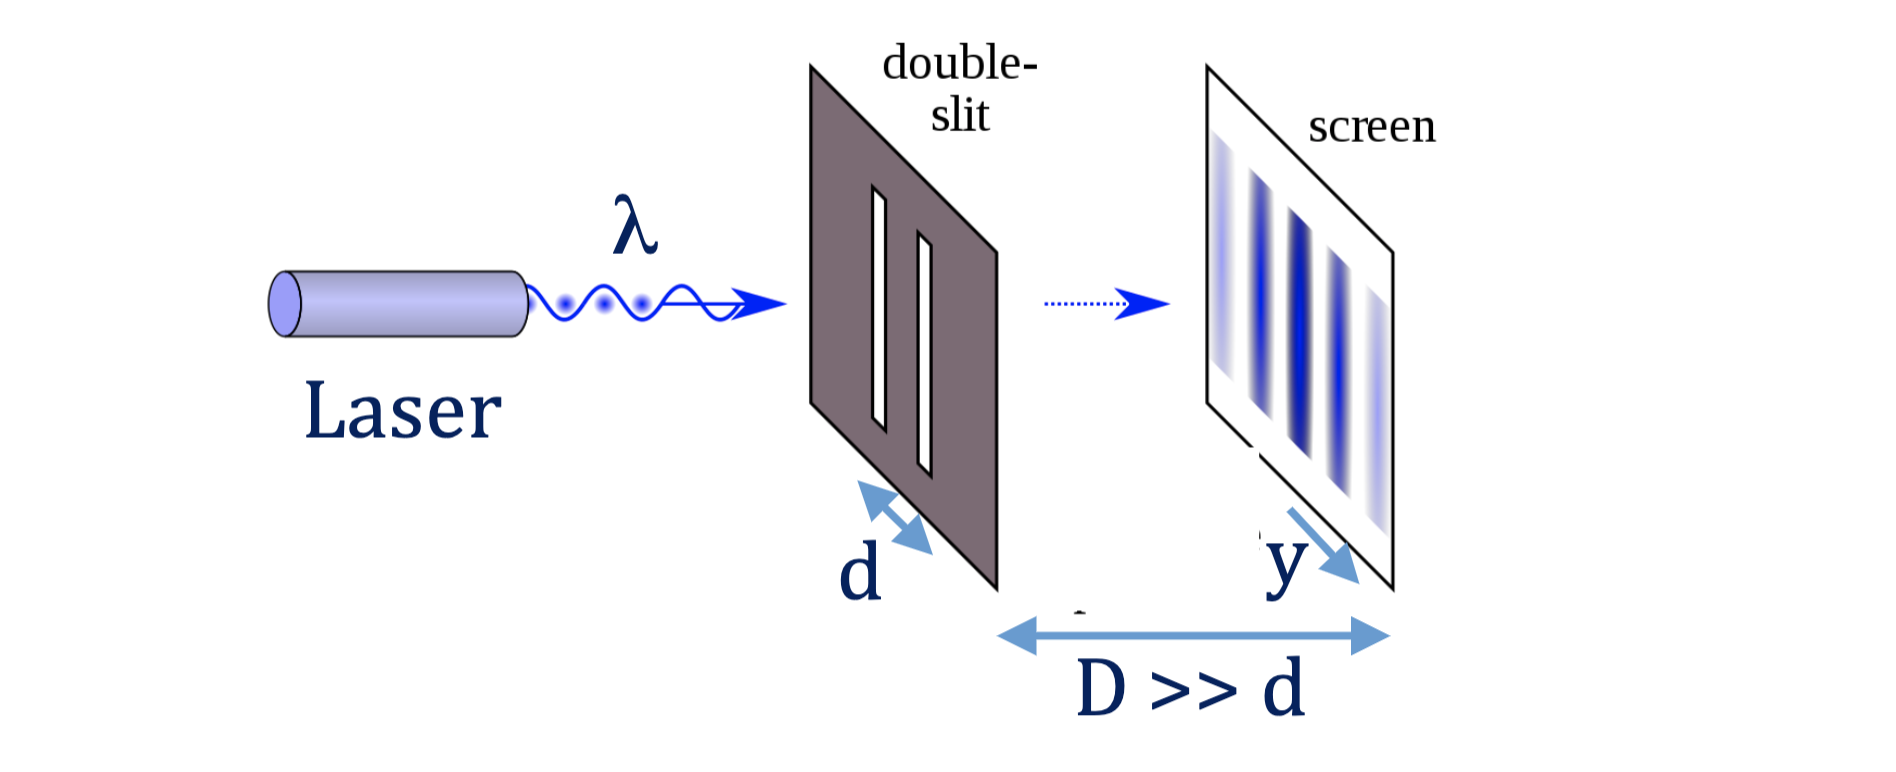
\includegraphics[scale=0.3]{diffraction}
\end{center}
From the image above, we obtain the expression for the intensity of the light as a function of $y$
$$ I(y) = 4 I_0 \cos ^2 \left( \frac{\pi Dy}{D\lambda }\right)$$



\section{Fourier Series and Transforms}
\subsection{Fourier Series Representation}
Consider a periodic function $f (x)$ with period $R$, that is $f (x + R) = f (x) $for all values of $x$. The functions $\sin(kx)$ and $\cos(kx)$ have periods $\frac{R}{n}$, where $n$ is an integer, so long as $kR = 2n\pi$. The Fourier series representation of this function is given as
$$ f(x) = \frac{a_0}{2} + \sum_{n=1}^{\infty} a_n \cos \left( \frac{2n\pi x}{R}\right) + \sum_{n=1}^{\infty} b_n \sin \left( \frac{2n\pi x}{R}\right)$$
where the values $a_0$, $a_n$, $b_n$ are given by
$$ a_0 = \frac{2}{R} \int \limits_{-R/2}^{R/2} f(x)  dx$$
$$ a_n = \frac{2}{R} \int \limits_{-R/2}^{R/2} f(x) \cos \left( \frac{2n\pi x}{R}\right) dx$$
$$ b_n = \frac{2}{R} \int \limits_{-R/2}^{R/2} f(x) \sin \left( \frac{2n\pi x}{R}\right) dx$$
\subsection{Complex Fourier Series}
The Fourier series of a function can also be represented in complex form:
$$f(x) = \frac{2\pi}{L} \sum_{n=-\infty}^{\infty} c_n e^{\frac{i2\pi n x}{L}}$$
$$f(x) = \frac{2\pi}{L} \sum_{n=-\infty}^{\infty} c_n \left( \cos \frac{2\pi n x}{L} + i \sin \frac{2\pi n x}{L}\right)$$
$$f(x) = \frac{2\pi}{L} c_0 + \frac{2\pi}{L} \sum_{n=-\infty}^{\infty} (c_n - c_{-n})  \cos \frac{2\pi n x}{L} + \frac{2\pi}{L} \sum_{n=-\infty}^{\infty} i (c_n - c_{-n}) \sin \frac{2\pi n x}{L}$$
In the final case, we separate the terms where $n=0$, $n < 0$, and $n > 0$. From this we can recognize that
$$ c_0 = A_0 \frac{L}{2\pi} \quad \quad c_n = (b_n - ia_n) \frac{L}{2\pi} \quad \quad c_{-n} = (b_n + ia_n) \frac{L}{2\pi} $$
\subsection{Fourier Transform}
In the cases prior, we were looking to represent only periodic functions with Fourier series. Consider a function $f(x)$ that is not periodic. We can define its Fourier Transform and Inverse Fourier Transform with the following integrals
$$ \tilde{\phi} (k) = \frac{1}{\sqrt{2\pi}} \int \limits_{-\infty}^{\infty} \phi(x) e^{-ikx} dx \quad \quad  \text{Fourier Transform} $$
$$ {\phi} (x) = \frac{1}{\sqrt{2\pi}} \int \limits_{-\infty}^{\infty} \tilde{\phi} (k) e^{-ikx} dk\quad \quad  \text{Inverse Fourier Transform} $$
\section{Position Momentum Uncertainty}

\section{Schrödinger Equation}
The one-dimensional time-dependent Schrödinger equation is given as the following:
$$i\frac{h}{2\pi} \frac{\partial \Psi}{\partial t} = \frac{h}{8\pi^2m} \frac{\partial^2 \Psi}{\partial x^2} + V\Psi $$


\end{document}
